\chapter{Temporal stabilization of clusters}

After clustering, we need to reassign colors to the clusters to stabilize them over time. \\
As mentioned before, the order in which clusters are determined at each moment is random, and the selection order of clusters is represented by a color.
Therefore, from the initial random color assignment, we aim to transition to a color assignment where two clusters of the same color share as many nodes (joints) as possible between moments.

This is because the random assignment of colors poses visualization issues for the graph.
It is possible that from one moment to the next, two clusters with many shared joints might have different colors, resulting in a visualization over time that appears as a continuous switching of colors. This could lead to a loss of continuity in the visual representation.
To stabilize clusters over time, ensuring that pairs of clusters colored from one moment to another share the highest number of common joints, we turn to the MaxWPM, seen in Section \ref{sec:MaxWPM}.

We have implemented two algorithms: a BF approach, where we compute the total weights of all possible permutations of color assignments and select the assignment with the maximum total weight, and the Hungarian Algorithm, a combinatorial optimization method that solves the assignment problem in polynomial time.

Since in our case the number of clusters is usually small, there are instances where the BF is more efficient.

\section{MaxWPM on clusters}
In our case, instead of having nodes connected by edges, we will have a slightly different situation.
Instead of the previously introduced nodes, we will have clusters, which are sets of nodes representing the joints of the skeleton, connected to each other by edges.\\  
Consider the clusters at time \textit{t} and the clusters at time \textit{t+1} as two distinct sets, so there will be no edges connecting clusters that belong to the same set.
Each cluster in one set must be connected by an edge to exactly one cluster in the other set, with the goal of maximizing the total weight of the edges.
The weight of an edge is equal to the number of nodes that the two clusters it is connecting have in common.\\
As previously mentioned, at this stage of the pipeline, we already have information about the joints belonging to various clusters and the colors of these clusters. However, we want to reassign colors to stabilize the visualization over time.
The previous clustering groups the joints into clusters and assigns them random colors, while in this phase of the pipeline, we optimize the color assignment.\\
We will start by analyzing the colors of the clusters at the initial frame and choose the best color assignment for the next frame.
Then will repeat this process iteratively until the last frame.


\subsection{A real application}
Let's consider a real-world scenario to understand how MaxWPM works in terms of visualization.
Suppose we have 20 nodes representing joints at time \textit{t} and 3 clusters labeled with different colors, as shown in Figure \ref{fig:clust_t}.
At time \textit{t+1}, there are the same 20 nodes as before but with 3 clusters changed but labeled using the same lexicographic order for the nodes (see Figure \ref{fig:clust_tplus1}). \\
Certainly, this clustering-based assignment cannot be regarded as the optimal assignment, as we still need to assess the \textit{3!} possible color assignments. \\
We know the colors of the clusters at time \textit{t}, and we want to assign colors to the clusters at time \textit{t+1}. \\
In Figure \ref{fig:clust_ass}, you can visually see all the possible color assignments, while in Table \ref{tab:table_clust}, all the values of common nodes for each color and the total weight of the matching are gathered.


\begin{figure}[H]
  \begin{subfigure}{\textwidth} % Adjust the width as needed
    \centering
    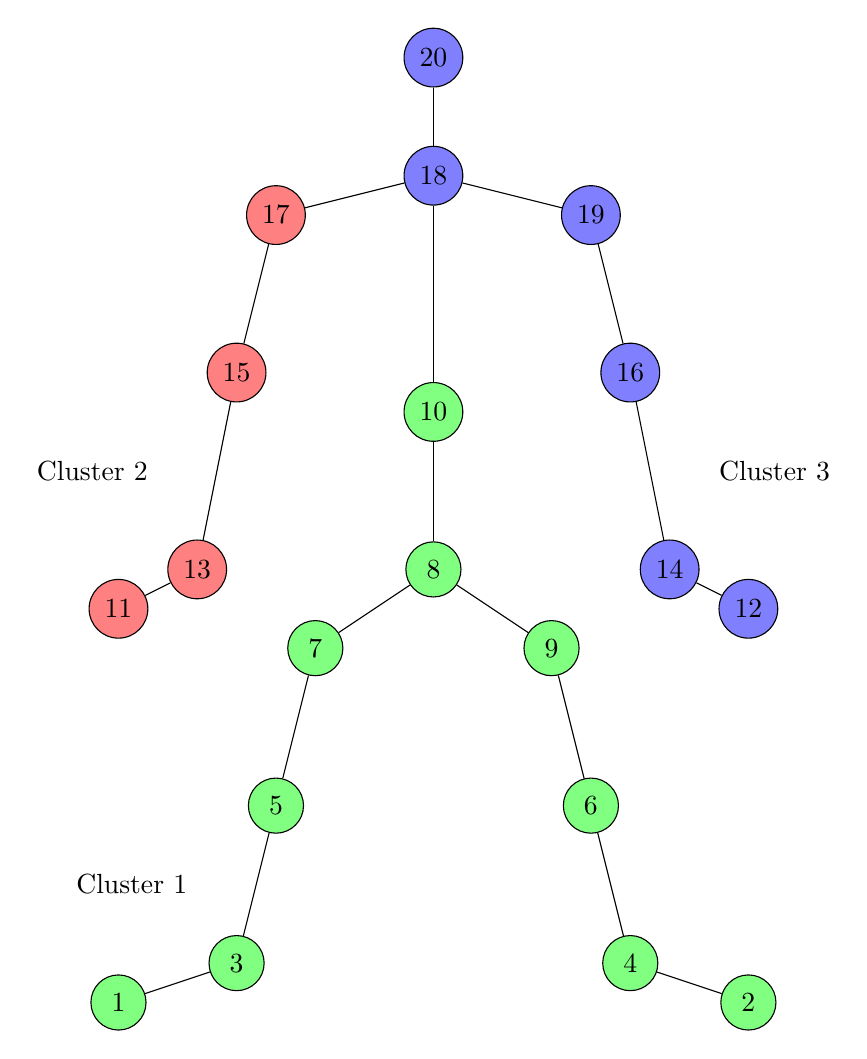
\begin{tikzpicture}
      \node[circle, draw, minimum size=0.7cm] (1) at (1,-9) [fill=green!50] {1};
      \node[circle, draw, minimum size=0.7cm] (2) at (9, -9) [fill=green!50] {2};
      \node[circle, draw, minimum size=0.7cm] (3) at (2.5,-8.5) [fill=green!50] {3};
      \node[circle, draw, minimum size=0.7cm] (4) at (7.5, -8.5) [fill=green!50] {4};
      \node[circle, draw, minimum size=0.7cm] (5) at (3,-6.5) [fill=green!50] {5};
      \node[circle, draw, minimum size=0.7cm] (6) at (7,-6.5) [fill=green!50] {6};
      \node[circle, draw, minimum size=0.7cm] (7) at (3.5,-4.5) [fill=green!50] {7};
      \node[circle, draw, minimum size=0.7cm] (8) at (5, -3.5) [fill=green!50] {8};
      \node[circle, draw, minimum size=0.7cm] (9) at (6.5,-4.5) [fill=green!50] {9};
      \node[circle, draw, minimum size=0.7cm] (10) at (5,-1.5) [fill=green!50] {10};
      \node[circle, draw, minimum size=0.7cm] (11) at (1,-4) [fill=red!50] {11};
      \node[circle, draw, minimum size=0.7cm] (12) at (9,-4) [fill=blue!50] {12};
      \node[circle, draw, minimum size=0.7cm] (13) at (2, -3.5) [fill=red!50] {13};
      \node[circle, draw, minimum size=0.7cm] (14) at (8, -3.5) [fill=blue!50] {14};
      \node[circle, draw, minimum size=0.7cm] (15) at (2.5,-1) [fill=red!50] {15};
      \node[circle, draw, minimum size=0.7cm] (16) at (7.5,-1) [fill=blue!50] {16};
      \node[circle, draw, minimum size=0.7cm] (17) at (3,1) [fill=red!50] {17};
      \node[circle, draw, minimum size=0.7cm] (18) at (5,1.5) [fill=blue!50] {18};
      \node[circle, draw, minimum size=0.7cm] (19) at (7,1) [fill=blue!50] {19};
      \node[circle, draw, minimum size=0.7cm] (20) at (5,3) [fill=blue!50] {20};
      \foreach \source/\dest/\label/\xshiftval in {20/18//0, 18/17//0, 18/19//0, 17/15//0, 15/13/Cluster 2/-45, 13/11//0, 19/16//0, 16/14/Cluster 3/45, 14/12//0, 18/10//0, 10/8//0, 8/7//0, 7/5//0, 5/3/Cluster 1/-45, 3/1//0, 8/9//0, 9/6//0, 6/4//0, 4/2//0}
        \path (\source) edge node[xshift=\xshiftval] {\label} (\dest);
    \end{tikzpicture}
    \caption{}
    \label{fig:clust_t}
  \end{subfigure}

  \vspace{1cm}

  \begin{subfigure}{\textwidth}
    \centering
    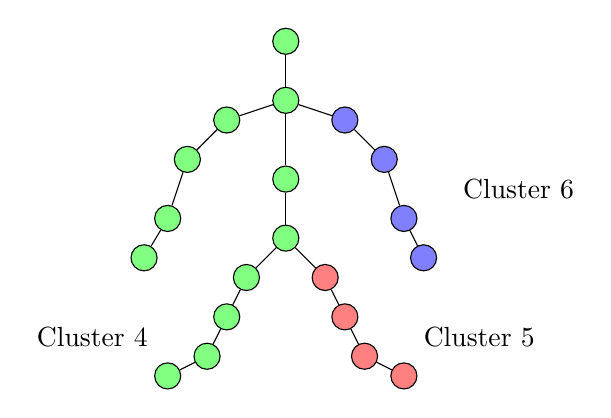
\begin{tikzpicture}
      \node[circle, draw, minimum size=0.3cm] (1) at (3.5,-1.25) [fill=green!50] {};
      \node[circle, draw, minimum size=0.3cm] (2) at (6.5, -1.25) [fill=red!50] {};
      \node[circle, draw, minimum size=0.3cm] (3) at (4,-1) [fill=green!50] {};
      \node[circle, draw, minimum size=0.3cm] (4) at (6, -1) [fill=red!50] {};
      \node[circle, draw, minimum size=0.3cm] (5) at (4.25,-0.5) [fill=green!50] {};
      \node[circle, draw, minimum size=0.3cm] (6) at (5.75,-0.5) [fill=red!50] {};
      \node[circle, draw, minimum size=0.3cm] (7) at (4.5,0) [fill=green!50] {};
      \node[circle, draw, minimum size=0.3cm] (8) at (5, 0.5) [fill=green!50] {};
      \node[circle, draw, minimum size=0.3cm] (9) at (5.5,0) [fill=red!50] {};
      \node[circle, draw, minimum size=0.3cm] (10) at (5,1.25) [fill=green!50] {};
      \node[circle, draw, minimum size=0.3cm] (11) at (3.2, 0.25) [fill=green!50] {};
      \node[circle, draw, minimum size=0.3cm] (12) at (6.75,0.25) [fill=blue!50] {};
      \node[circle, draw, minimum size=0.3cm] (13) at (3.5, 0.75) [fill=green!50] {};
      \node[circle, draw, minimum size=0.3cm] (14) at (6.5, 0.75) [fill=blue!50] {};
      \node[circle, draw, minimum size=0.3cm] (15) at (3.75,1.5) [fill=green!50] {};
      \node[circle, draw, minimum size=0.3cm] (16) at (6.25,1.5) [fill=blue!50] {};
      \node[circle, draw, minimum size=0.3cm] (17) at (4.25,2) [fill=green!50] {};
      \node[circle, draw, minimum size=0.3cm] (18) at (5,2.25) [fill=green!50] {};
      \node[circle, draw, minimum size=0.3cm] (19) at (5.75,2) [fill=blue!50] {};
      \node[circle, draw, minimum size=0.3cm] (20) at (5,3) [fill=green!50] {};  
      \foreach \source/\dest/\label/\xshiftval in {20/18//0, 18/17//0, 18/19//0, 17/15//0, 15/13//-45, 13/11//0, 19/16//0, 16/14/Cluster 6/45, 14/12//0, 18/10//0, 10/8//0, 8/7//0, 7/5//0, 5/3/Cluster 4/-45, 3/1//0, 8/9//0, 9/6//0, 6/4/Cluster 5/45, 4/2//0}
        \path (\source) edge node[xshift=\xshiftval] {\label} (\dest);
    \end{tikzpicture}
    \caption{}
    \label{fig:clust_tplus1}
  \end{subfigure}
  \caption{Color assignment at time \textit{t} (a) and \textit{t+1} (b)}
\end{figure}


\begin{figure}[H]
  \centering
  \begin{subfigure}{0.3\textwidth}
    \centering
    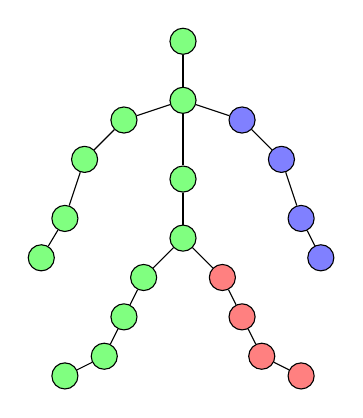
\begin{tikzpicture}[every node/.style={circle, draw, minimum size=0.1cm}]
      \node (1) at (3.5,-1.25) [fill=green!50] {};
      \node (2) at (6.5, -1.25) [fill=red!50] {};
      \node (3) at (4,-1) [fill=green!50] {};
      \node (4) at (6, -1) [fill=red!50] {};
      \node (5) at (4.25,-0.5) [fill=green!50] {};
      \node (6) at (5.75,-0.5) [fill=red!50] {};
      \node (7) at (4.5,0) [fill=green!50] {};
      \node (8) at (5, 0.5) [fill=green!50] {};
      \node (9) at (5.5,0) [fill=red!50] {};
      \node (10) at (5,1.25) [fill=green!50] {};
      \node (11) at (3.2, 0.25) [fill=green!50] {};
      \node (12) at (6.75,0.25) [fill=blue!50] {};
      \node (13) at (3.5, 0.75) [fill=green!50] {};
      \node (14) at (6.5, 0.75) [fill=blue!50] {};
      \node (15) at (3.75,1.5) [fill=green!50] {};
      \node (16) at (6.25,1.5) [fill=blue!50] {};
      \node (17) at (4.25,2) [fill=green!50] {};
      \node (18) at (5,2.25) [fill=green!50] {};
      \node (19) at (5.75,2) [fill=blue!50] {};
      \node (20) at (5,3) [fill=green!50] {};  
      \foreach \source/\dest in {20/18, 18/17, 18/19, 17/15, 15/13, 13/11, 19/16, 16/14, 14/12, 18/10, 10/8, 8/7, 7/5, 5/3, 3/1, 8/9, 9/6, 6/4, 4/2}
        \path (\source) edge (\dest);
    \end{tikzpicture}
      \caption{}
  \end{subfigure}
  \begin{subfigure}{0.3\textwidth}
    \centering
    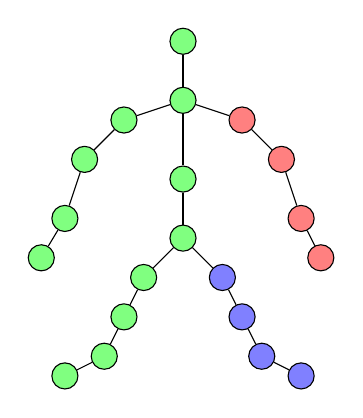
\begin{tikzpicture}[every node/.style={circle, draw, minimum size=0.1cm}]
      \node (1) at (3.5,-1.25) [fill=green!50] {};
      \node (2) at (6.5, -1.25) [fill=blue!50] {};
      \node (3) at (4,-1) [fill=green!50] {};
      \node (4) at (6, -1) [fill=blue!50] {};
      \node (5) at (4.25,-0.5) [fill=green!50] {};
      \node (6) at (5.75,-0.5) [fill=blue!50] {};
      \node (7) at (4.5,0) [fill=green!50] {};
      \node (8) at (5, 0.5) [fill=green!50] {};
      \node (9) at (5.5,0) [fill=blue!50] {};
      \node (10) at (5,1.25) [fill=green!50] {};
      \node (11) at (3.2, 0.25) [fill=green!50] {};
      \node (12) at (6.75,0.25) [fill=red!50] {};
      \node (13) at (3.5, 0.75) [fill=green!50] {};
      \node (14) at (6.5, 0.75) [fill=red!50] {};
      \node (15) at (3.75,1.5) [fill=green!50] {};
      \node (16) at (6.25,1.5) [fill=red!50] {};
      \node (17) at (4.25,2) [fill=green!50] {};
      \node (18) at (5,2.25) [fill=green!50] {};
      \node (19) at (5.75,2) [fill=red!50] {};
      \node (20) at (5,3) [fill=green!50] {};  
      \foreach \source/\dest in {20/18, 18/17, 18/19, 17/15, 15/13, 13/11, 19/16, 16/14, 14/12, 18/10, 10/8, 8/7, 7/5, 5/3, 3/1, 8/9, 9/6, 6/4, 4/2}
        \path (\source) edge (\dest);
    \end{tikzpicture}
      \caption{}
  \end{subfigure}
  \begin{subfigure}{0.3\textwidth}
    \centering
    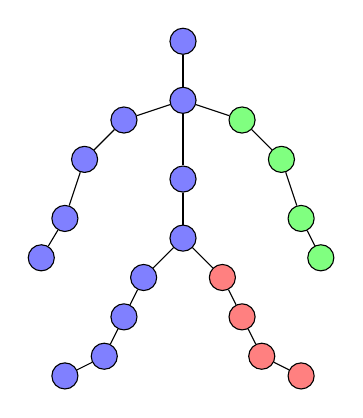
\begin{tikzpicture}[every node/.style={circle, draw, minimum size=0.1cm}]
      \node (1) at (3.5,-1.25) [fill=blue!50] {};
      \node (2) at (6.5, -1.25) [fill=red!50] {};
      \node (3) at (4,-1) [fill=blue!50] {};
      \node (4) at (6, -1) [fill=red!50] {};
      \node (5) at (4.25,-0.5) [fill=blue!50] {};
      \node (6) at (5.75,-0.5) [fill=red!50] {};
      \node (7) at (4.5,0) [fill=blue!50] {};
      \node (8) at (5, 0.5) [fill=blue!50] {};
      \node (9) at (5.5,0) [fill=red!50] {};
      \node (10) at (5,1.25) [fill=blue!50] {};
      \node (11) at (3.2, 0.25) [fill=blue!50] {};
      \node (12) at (6.75,0.25) [fill=green!50] {};
      \node (13) at (3.5, 0.75) [fill=blue!50] {};
      \node (14) at (6.5, 0.75) [fill=green!50] {};
      \node (15) at (3.75,1.5) [fill=blue!50] {};
      \node (16) at (6.25,1.5) [fill=green!50] {};
      \node (17) at (4.25,2) [fill=blue!50] {};
      \node (18) at (5,2.25) [fill=blue!50] {};
      \node (19) at (5.75,2) [fill=green!50] {};
      \node (20) at (5,3) [fill=blue!50] {};  
      \foreach \source/\dest in {20/18, 18/17, 18/19, 17/15, 15/13, 13/11, 19/16, 16/14, 14/12, 18/10, 10/8, 8/7, 7/5, 5/3, 3/1, 8/9, 9/6, 6/4, 4/2}
        \path (\source) edge (\dest);
    \end{tikzpicture}
      \caption{}
  \end{subfigure}
  
  \vspace{1cm} % Spazio vuoto tra le righe
  
  \begin{subfigure}{0.3\textwidth}
    \centering
    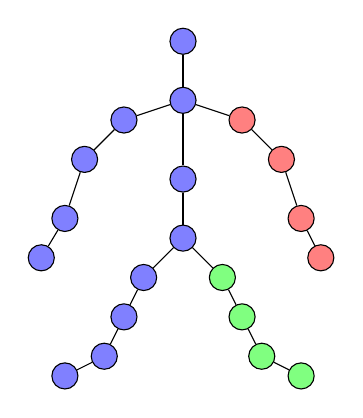
\begin{tikzpicture}[every node/.style={circle, draw, minimum size=0.1cm}]
      \node (1) at (3.5,-1.25) [fill=blue!50] {};
      \node (2) at (6.5, -1.25) [fill=green!50] {};
      \node (3) at (4,-1) [fill=blue!50] {};
      \node (4) at (6, -1) [fill=green!50] {};
      \node (5) at (4.25,-0.5) [fill=blue!50] {};
      \node (6) at (5.75,-0.5) [fill=green!50] {};
      \node (7) at (4.5,0) [fill=blue!50] {};
      \node (8) at (5, 0.5) [fill=blue!50] {};
      \node (9) at (5.5,0) [fill=green!50] {};
      \node (10) at (5,1.25) [fill=blue!50] {};
      \node (11) at (3.2, 0.25) [fill=blue!50] {};
      \node (12) at (6.75,0.25) [fill=red!50] {};
      \node (13) at (3.5, 0.75) [fill=blue!50] {};
      \node (14) at (6.5, 0.75) [fill=red!50] {};
      \node (15) at (3.75,1.5) [fill=blue!50] {};
      \node (16) at (6.25,1.5) [fill=red!50] {};
      \node (17) at (4.25,2) [fill=blue!50] {};
      \node (18) at (5,2.25) [fill=blue!50] {};
      \node (19) at (5.75,2) [fill=red!50] {};
      \node (20) at (5,3) [fill=blue!50] {};  
      \foreach \source/\dest in {20/18, 18/17, 18/19, 17/15, 15/13, 13/11, 19/16, 16/14, 14/12, 18/10, 10/8, 8/7, 7/5, 5/3, 3/1, 8/9, 9/6, 6/4, 4/2}
        \path (\source) edge (\dest);
    \end{tikzpicture}
      \caption{}
  \end{subfigure}
  \begin{subfigure}{0.3\textwidth}
    \centering
    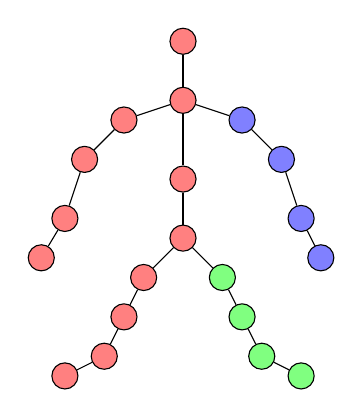
\begin{tikzpicture}[every node/.style={circle, draw, minimum size=0.1cm}]
      \node (1) at (3.5,-1.25) [fill=red!50] {};
      \node (2) at (6.5, -1.25) [fill=green!50] {};
      \node (3) at (4,-1) [fill=red!50] {};
      \node (4) at (6, -1) [fill=green!50] {};
      \node (5) at (4.25,-0.5) [fill=red!50] {};
      \node (6) at (5.75,-0.5) [fill=green!50] {};
      \node (7) at (4.5,0) [fill=red!50] {};
      \node (8) at (5, 0.5) [fill=red!50] {};
      \node (9) at (5.5,0) [fill=green!50] {};
      \node (10) at (5,1.25) [fill=red!50] {};
      \node (11) at (3.2, 0.25) [fill=red!50] {};
      \node (12) at (6.75,0.25) [fill=blue!50] {};
      \node (13) at (3.5, 0.75) [fill=red!50] {};
      \node (14) at (6.5, 0.75) [fill=blue!50] {};
      \node (15) at (3.75,1.5) [fill=red!50] {};
      \node (16) at (6.25,1.5) [fill=blue!50] {};
      \node (17) at (4.25,2) [fill=red!50] {};
      \node (18) at (5,2.25) [fill=red!50] {};
      \node (19) at (5.75,2) [fill=blue!50] {};
      \node (20) at (5,3) [fill=red!50] {};  
      \foreach \source/\dest in {20/18, 18/17, 18/19, 17/15, 15/13, 13/11, 19/16, 16/14, 14/12, 18/10, 10/8, 8/7, 7/5, 5/3, 3/1, 8/9, 9/6, 6/4, 4/2}
        \path (\source) edge (\dest);
    \end{tikzpicture}
      \caption{}
  \end{subfigure}
  \begin{subfigure}{0.3\textwidth}
    \centering
    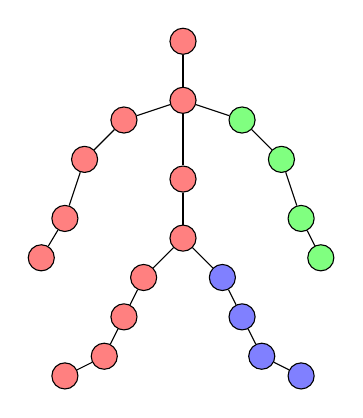
\begin{tikzpicture}[every node/.style={circle, draw, minimum size=0.1cm}]
      \node (1) at (3.5,-1.25) [fill=red!50] {};
      \node (2) at (6.5, -1.25) [fill=blue!50] {};
      \node (3) at (4,-1) [fill=red!50] {};
      \node (4) at (6, -1) [fill=blue!50] {};
      \node (5) at (4.25,-0.5) [fill=red!50] {};
      \node (6) at (5.75,-0.5) [fill=blue!50] {};
      \node (7) at (4.5,0) [fill=red!50] {};
      \node (8) at (5, 0.5) [fill=red!50] {};
      \node (9) at (5.5,0) [fill=blue!50] {};
      \node (10) at (5,1.25) [fill=red!50] {};
      \node (11) at (3.2, 0.25) [fill=red!50] {};
      \node (12) at (6.75,0.25) [fill=green!50] {};
      \node (13) at (3.5, 0.75) [fill=red!50] {};
      \node (14) at (6.5, 0.75) [fill=green!50] {};
      \node (15) at (3.75,1.5) [fill=red!50] {};
      \node (16) at (6.25,1.5) [fill=green!50] {};
      \node (17) at (4.25,2) [fill=red!50] {};
      \node (18) at (5,2.25) [fill=red!50] {};
      \node (19) at (5.75,2) [fill=green!50] {};
      \node (20) at (5,3) [fill=red!50] {};  
      \foreach \source/\dest in {20/18, 18/17, 18/19, 17/15, 15/13, 13/11, 19/16, 16/14, 14/12, 18/10, 10/8, 8/7, 7/5, 5/3, 3/1, 8/9, 9/6, 6/4, 4/2}
        \path (\source) edge (\dest);
    \end{tikzpicture}
      \caption{}
  \end{subfigure}

  \vspace{0.5cm} % Spazio vuoto tra le righe
  
  \caption{Possible color assignments at time \textit{t+1}}
  \label{fig:clust_ass}
\end{figure}



\begin{table}[H]
  \centering
  \begin{tabular}{|c|c|c|c|c|}
    \hline
   \textbf{Assignment} & \textbf{Red match} & \textbf{Blue match} & \textbf{Green match} & \textbf{Utility Value} \\
    \hline
    (a) & 0 & 4 & 6 & 10 \\
    \hline
    (b) & 0 & 0 & 6 & 6 \\
    \hline
    (c) & 0 & 2 & 0 & 2 \\
    \hline
    (d) & 0 & 2 & 4 & 6 \\
    \hline
    (e) & 4 & 4 & 4 & 12 \\
    \hline
    (f) & 4 & 0 & 0 & 4 \\
    \hline
  \end{tabular}
  
  \vspace{0.5cm} % Spazio vuoto tra le righe
  
  \caption{Matching weights for the 6 assignments}
  \label{tab:table_clust}
\end{table}
 
From Table \ref{tab:table_clust}, it can be observed that assignment (e) has the highest utility value.
Additionally, even visually, it can be noticed that it is the most consistent assignment compared to the one at time \textit{t}.
\\

From the perspective of Bipartite Matching, we can consider the clusters from Figure \ref{fig:clust_t} in the first partition, while in the second partition, we can consider the clusters from Figure \ref{fig:clust_tplus1}.
As mentioned earlier, the weight of an edge is equivalent to the number of nodes that the two clusters being connected by that edge have in common. \\
The following figure shows the matching with the utility value for every possible assignment and the colored ones for the optimal one.



\begin{figure}[H]
  \centering
  \begin{minipage}{0.45\textwidth}
    \centering
    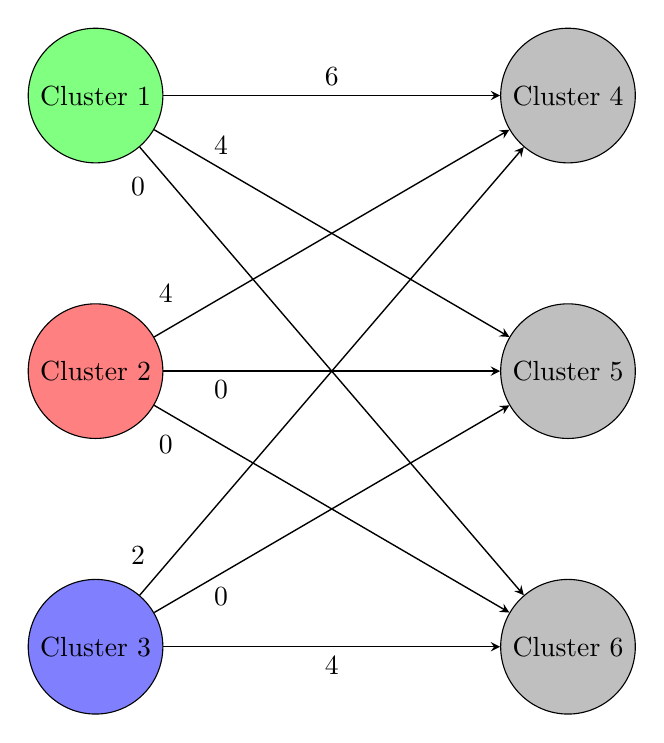
\begin{tikzpicture}
      \node[circle, draw, minimum size=1cm, fill=green!50] (1) at (2,-6.5) {Cluster 1};
      \node[circle, draw, minimum size=1cm, fill=red!50] (2) at (2, -10) {Cluster 2};
      \node[circle, draw, minimum size=1cm, fill=blue!50] (3) at (2,-13.5) {Cluster 3};
      \node[circle, draw, minimum size=1cm, fill=gray!50] (4) at (8, -6.5) {Cluster 4};
      \node[circle, draw, minimum size=1cm, fill=gray!50] (5) at (8,-10) {Cluster 5};
      \node[circle, draw, minimum size=1cm, fill=gray!50] (6) at (8,-13.5) {Cluster 6};
      
      \foreach \source/\dest/\label/\position/\yshiftval/\xshiftval/\edgecolor in {
        1/4/6/above/0/0/black, 1/5/4/above/25/-40/black, 1/6/0/above/60/-70/black,
        2/4/4/below/-15/-60/black, 2/5/0/below/0/-40/black, 2/6/0/below/30/-60/black,
        3/4/2/below/-60/-70/black, 3/5/0/below/-25/-40/black, 3/6/4/below/0/0/black}
        \path (\source) edge[\edgecolor, ->,>=stealth, line width=0.5pt] node[\position, yshift=\yshiftval, xshift=\xshiftval, black] {\label} (\dest);
    \end{tikzpicture}
  \end{minipage}
  \hfill
  \begin{minipage}{0.45\textwidth}
    \centering
    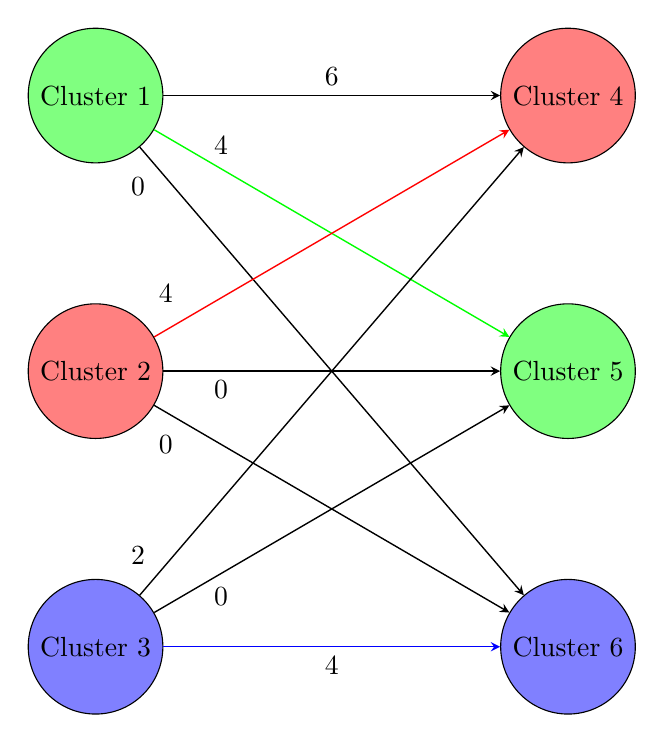
\begin{tikzpicture}
      \node[circle, draw, minimum size=1cm, fill=green!50] (1) at (2,-6.5) {Cluster 1};
      \node[circle, draw, minimum size=1cm, fill=red!50] (2) at (2, -10) {Cluster 2};
      \node[circle, draw, minimum size=1cm, fill=blue!50] (3) at (2,-13.5) {Cluster 3};
      \node[circle, draw, minimum size=1cm, fill=red!50] (4) at (8, -6.5) {Cluster 4};
      \node[circle, draw, minimum size=1cm, fill=green!50] (5) at (8,-10) {Cluster 5};
      \node[circle, draw, minimum size=1cm, fill=blue!50] (6) at (8,-13.5) {Cluster 6};
      
      \foreach \source/\dest/\label/\position/\yshiftval/\xshiftval/\edgecolor in {
        1/4/6/above/0/0/black, 1/5/4/above/25/-40/green, 1/6/0/above/60/-70/black,
        2/4/4/below/-15/-60/red, 2/5/0/below/0/-40/black, 2/6/0/below/30/-60/black,
        3/4/2/below/-60/-70/black, 3/5/0/below/-25/-40/black, 3/6/4/below/0/0/blue}
        \path (\source) edge[\edgecolor, ->,>=stealth, line width=0.5pt] node[\position, yshift=\yshiftval, xshift=\xshiftval, black] {\label} (\dest);
    \end{tikzpicture}
  \end{minipage}
  \caption{Bipartite Matching from instant \textit{t} to instant \textit{t+1}}
  \label{fig:clust_match}
\end{figure}



\subsection{Brute Force Algorithm application}
As presented in Section \ref{sec:bf}, a BF approach for choosing an option based on the minimum sum of utility values of a graph involves exhaustively evaluating every possible combination of options to find the one with the highest total weight. 
This method consists of:
\begin{enumerate}
  \item Generating all possible combinations: Enumerate all possible subsets or combinations of options within the graph.
  \item Calculating the sum of weights: For each combination, compute the total weight by summing the weights of the selected options.
  \item Comparing and selecting: Identify the combination with the minimum total weight as the optimal choice.
\end{enumerate}
The Table \ref{tab:bf_alg} is a clear example of this approach. \\   

\begin{table}[H]
  \centering
  \begin{minipage}{0.3\textwidth}
    \centering
    \begin{tabular}{|>{\centering\arraybackslash}m{0.6cm}|>{\centering\arraybackslash}m{0.6cm}|>{\centering\arraybackslash}m{0.6cm}|}
      \hline
      \cellcolor{green!50}-6 & -4 & 0 \\
      \hline
      -4 & \cellcolor{green!50}0 & 0 \\
      \hline
      -2 & 0 & \cellcolor{green!50}-4 \\
      \hline
    \end{tabular}
    \caption*{(a)}
  \end{minipage}
  \hfill
  \begin{minipage}{0.3\textwidth}
    \centering
    \begin{tabular}{|>{\centering\arraybackslash}m{0.6cm}|>{\centering\arraybackslash}m{0.6cm}|>{\centering\arraybackslash}m{0.6cm}|}
      \hline
      \cellcolor{green!50}-6 & -4 & 0 \\
      \hline
      -4 & 0 & \cellcolor{green!50}0 \\
      \hline
      -2 & \cellcolor{green!50}0 & -4 \\
      \hline
    \end{tabular}
    \caption*{(b)}
  \end{minipage}
  \hfill
  \begin{minipage}{0.3\textwidth}
    \centering
    \begin{tabular}{|>{\centering\arraybackslash}m{0.6cm}|>{\centering\arraybackslash}m{0.6cm}|>{\centering\arraybackslash}m{0.6cm}|}
      \hline
      -6 & -4 & \cellcolor{green!50}0 \\
      \hline
      -4 & \cellcolor{green!50}0 & 0 \\
      \hline
      \cellcolor{green!50}-2 & 0 & -4 \\
      \hline
    \end{tabular}
    \caption*{(c)}
  \end{minipage}

  \vspace{10pt}

  \begin{minipage}{0.3\textwidth}
    \centering
    \begin{tabular}{|>{\centering\arraybackslash}m{0.6cm}|>{\centering\arraybackslash}m{0.6cm}|>{\centering\arraybackslash}m{0.6cm}|}
      \hline
      -6 & \cellcolor{green!50}-4 & 0 \\
      \hline
      -4 & 0 & \cellcolor{green!50}0 \\
      \hline
      \cellcolor{green!50}-2 & 0 & -4 \\
      \hline
    \end{tabular}
    \caption*{(d)}
  \end{minipage}
  \hfill
  \begin{minipage}{0.3\textwidth}
    \centering  
    \begin{tabular}{|>{\centering\arraybackslash}m{0.6cm}|>{\centering\arraybackslash}m{0.6cm}|>{\centering\arraybackslash}m{0.6cm}|}
      \hline
      -6 & \cellcolor{green!50}-4 & 0 \\
      \hline
      \cellcolor{green!50}-4 & 0 & 0 \\
      \hline
      -2 & 0 & \cellcolor{green!50}-4 \\
      \hline
    \end{tabular}
    \caption*{(e)}
  \end{minipage}
  \hfill
  \begin{minipage}{0.3\textwidth}
    \centering
    \begin{tabular}{|>{\centering\arraybackslash}m{0.6cm}|>{\centering\arraybackslash}m{0.6cm}|>{\centering\arraybackslash}m{0.6cm}|}
      \hline
      -6 & -4 & \cellcolor{green!50}0 \\
      \hline
      \cellcolor{green!50}-4 & 0 & 0 \\
      \hline
      -2 & \cellcolor{green!50}0 & -4 \\
      \hline
    \end{tabular}
    \caption*{(f)}
  \end{minipage}
  \caption{Real application of the BF Algorithm}
  \label{tab:bf_alg}
\end{table}


BF approach guarantees finding the best option, it can be computationally expensive, especially for large graphs.
As we can see, here we have the computation of all the \textit{n!} permutations and the minimum one is (e).

\subsection{Hungarian Matching Algorithm application}
Another approach consists in applying the Hungarian Algorithm which is a combinatorial optimization algorithm that also solves the assignment problem.\\
Now let's see the previous example solved with this algorithm in the Table \ref{tab:hung_alg_appl}: 
\begin{enumerate}
  \item[(a)] From the original table that describes the utility value associated for every assignment
  \item[(b)] Invert each element to obtain the cost value of every assignment, since we want to minimize it 
  \item[(c)] Now, subtract the smallest value for each row
  \item[(d)] Subtract the smallest value for each column 
  \item[(e)] Draw the minimum number of lines to cover the rows and columns that have 0 entries
            There are 3 rows this means that we can find the optimal solution, since there are 3 rows
  \item[(f)] Starting from the top-left corner select the zero that does not cover other zeros in any uncovered row or column
  \item[(g)] Select cells that does cover the less amount of 0 for each row and has not the column already covered, so the zero in the bottom right corner
  \item[(h)] Select the remaining cell that isn't already covered by any column
  \item[(i)] Restore the original cost matrix 
\end{enumerate}

\begin{table}[H]
  \centering
  \begin{minipage}{0.3\textwidth}
    \centering
    \begin{tabular}{|>{\centering\arraybackslash}m{0.6cm}|>{\centering\arraybackslash}m{0.6cm}|>{\centering\arraybackslash}m{0.6cm}|}
      \hline
      6 & 4 & 0 \\
      \hline
      4 & 0 & 0 \\
      \hline
      2 & 0 & 4 \\
      \hline
    \end{tabular}
    \caption*{(a)}
  \end{minipage}
  \hfill
  \begin{minipage}{0.3\textwidth}
    \centering
    \begin{tabular}{|>{\centering\arraybackslash}m{0.6cm}|>{\centering\arraybackslash}m{0.6cm}|>{\centering\arraybackslash}m{0.6cm}|}
      \hline
      -6 & -4 & 0 \\
      \hline
      -4 & 0 & 0 \\
      \hline
      -2 & 0 & -4 \\
      \hline
    \end{tabular}
    \caption*{(b)}
  \end{minipage}
  \hfill
  \begin{minipage}{0.3\textwidth}
    \centering
    \begin{tabular}{|>{\centering\arraybackslash}m{0.6cm}|>{\centering\arraybackslash}m{0.6cm}|>{\centering\arraybackslash}m{0.6cm}|}
      \hline
      0 & 2 & 6 \\
      \hline
      0 & 4 & 4 \\
      \hline
      2 & 4 & 0 \\
      \hline
    \end{tabular}
    \caption*{(c)}
  \end{minipage}

  \vspace{10pt}

  \begin{minipage}{0.3\textwidth}
    \centering
    \begin{tabular}{|>{\centering\arraybackslash}m{0.6cm}|>{\centering\arraybackslash}m{0.6cm}|>{\centering\arraybackslash}m{0.6cm}|}
      \hline
      0 & 0 & 6 \\
      \hline
      0 & 2 & 4 \\
      \hline
      2 & 2 & 0 \\
      \hline
    \end{tabular}
    \caption*{(d)}
  \end{minipage}
  \hfill
  \begin{minipage}{0.3\textwidth}
    \centering
    \begin{tabular}{|>{\centering\arraybackslash}m{0.6cm}|>{\centering\arraybackslash}m{0.6cm}|>{\centering\arraybackslash}m{0.6cm}|}
      \hline
      \cellcolor{gray!25} 0 & \cellcolor{gray!25} 0 & \cellcolor{gray!25} 6 \\
      \hline
      \cellcolor{gray!25} 0 & \cellcolor{gray!25} 2 & \cellcolor{gray!25} 4 \\
      \hline
      2 & 2 & \cellcolor{gray!25} 0 \\
      \hline
    \end{tabular}
    \caption*{(e)}
  \end{minipage}
  \hfill
  \begin{minipage}{0.3\textwidth}
    \centering
    \begin{tabular}{|>{\centering\arraybackslash}m{0.6cm}|>{\centering\arraybackslash}m{0.6cm}|>{\centering\arraybackslash}m{0.6cm}|}
      \hline
      \cellcolor{gray!25} 0 & \cellcolor{gray!25} 0 & \cellcolor{gray!25} 6 \\
      \hline
      \cellcolor{green!50} 0 & \cellcolor{gray!25} 2 & \cellcolor{gray!25} 4 \\
      \hline
      2 & 2 & \cellcolor{gray!25} 0 \\
      \hline
    \end{tabular}
    \caption*{(f)}
  \end{minipage}

  \vspace{10pt}

  \begin{minipage}{0.3\textwidth}
    \centering
    \begin{tabular}{|>{\centering\arraybackslash}m{0.6cm}|>{\centering\arraybackslash}m{0.6cm}|>{\centering\arraybackslash}m{0.6cm}|}
      \hline
      \cellcolor{gray!25} 0 & \cellcolor{gray!25} 0 & \cellcolor{gray!25} 6 \\
      \hline
      \cellcolor{green!50} 0 & \cellcolor{gray!25} 2 & \cellcolor{gray!25} 4 \\
      \hline
      2 & 2 & \cellcolor{green!50} 0 \\
      \hline
    \end{tabular}
    \caption*{(g)}
  \end{minipage}
  \hfill
  \begin{minipage}{0.3\textwidth}
    \centering
    \begin{tabular}{|>{\centering\arraybackslash}m{0.6cm}|>{\centering\arraybackslash}m{0.6cm}|>{\centering\arraybackslash}m{0.6cm}|}
      \hline
      0 & \cellcolor{green!50} 0 & 6 \\
      \hline
      \cellcolor{green!50} 0 & 2 & 4 \\
      \hline
      2 & 2 & \cellcolor{green!50} 0 \\
      \hline
    \end{tabular}
    \caption*{(h)}
  \end{minipage}
  \hfill
  \begin{minipage}{0.3\textwidth}
    \centering
    \begin{tabular}{|>{\centering\arraybackslash}m{0.6cm}|>{\centering\arraybackslash}m{0.6cm}|>{\centering\arraybackslash}m{0.6cm}|}
      \hline
      6 & \cellcolor{green!50} 4 & 0 \\
      \hline
      \cellcolor{green!50} 4 & 0 & 0 \\
      \hline
      2 & 0 & \cellcolor{green!50} 4 \\
      \hline
    \end{tabular}
    \caption*{(i)}
  \end{minipage}
  \caption{Application of the Hungarian Algorithm to clusters stabilization}
  \label{tab:hung_alg_appl}
\end{table}

Both these methods provide the same results but lead to different complexities.

\subsection{Clustering Transition Smoothing}

After achieving cluster stabilization at the interframe level, a persistent issue remains. 
Despite the smoothness of actual movements, the evolution of clusters on joints appears inflexible 
and primarily optimized from one frame to the next, 
without considering the temporal progression of clusters in terms of identifying the source of the movement.

For the sole purpose of visualization, a delaying and smoothing procedure has been implemented as follows:
\begin{enumerate}
  \item Apply only every $k = \frac{1}{4}framerate$ time instant otherwise keep the previous clustering
  \item Calculate the difference between the sets representing clusters at time t+1 and clusters at time t is computed.
  \item Weighted degree centrality is applied to the nodes within each cluster in the resulting set, and the maximum value is selected.
  \item For each cluster, update the label of the node with the highest weighted degree centrality.
\end{enumerate}

By parameterizing $k$ this process appropriately to ensure that clusters do not undergo excessive changes during this time interval, an oscillating effect is achieved. 
This effect propagates the cluster across the connected nodes that belong to it, thereby making any potential origin of the movement more conspicuous.

\subsection{Stabilization Results}
In this first example, in Figure \ref{fig:stabilization_results}, we can observe the results of stabilization between two different instants in time. 
In (a), the preceding time instant is visible, while (b) showcases the subsequent time instant in an unstabilized state. 
In (c) instead, the subsequent time instant with clusters stabilized.

\begin{figure}[H]
  \centering
  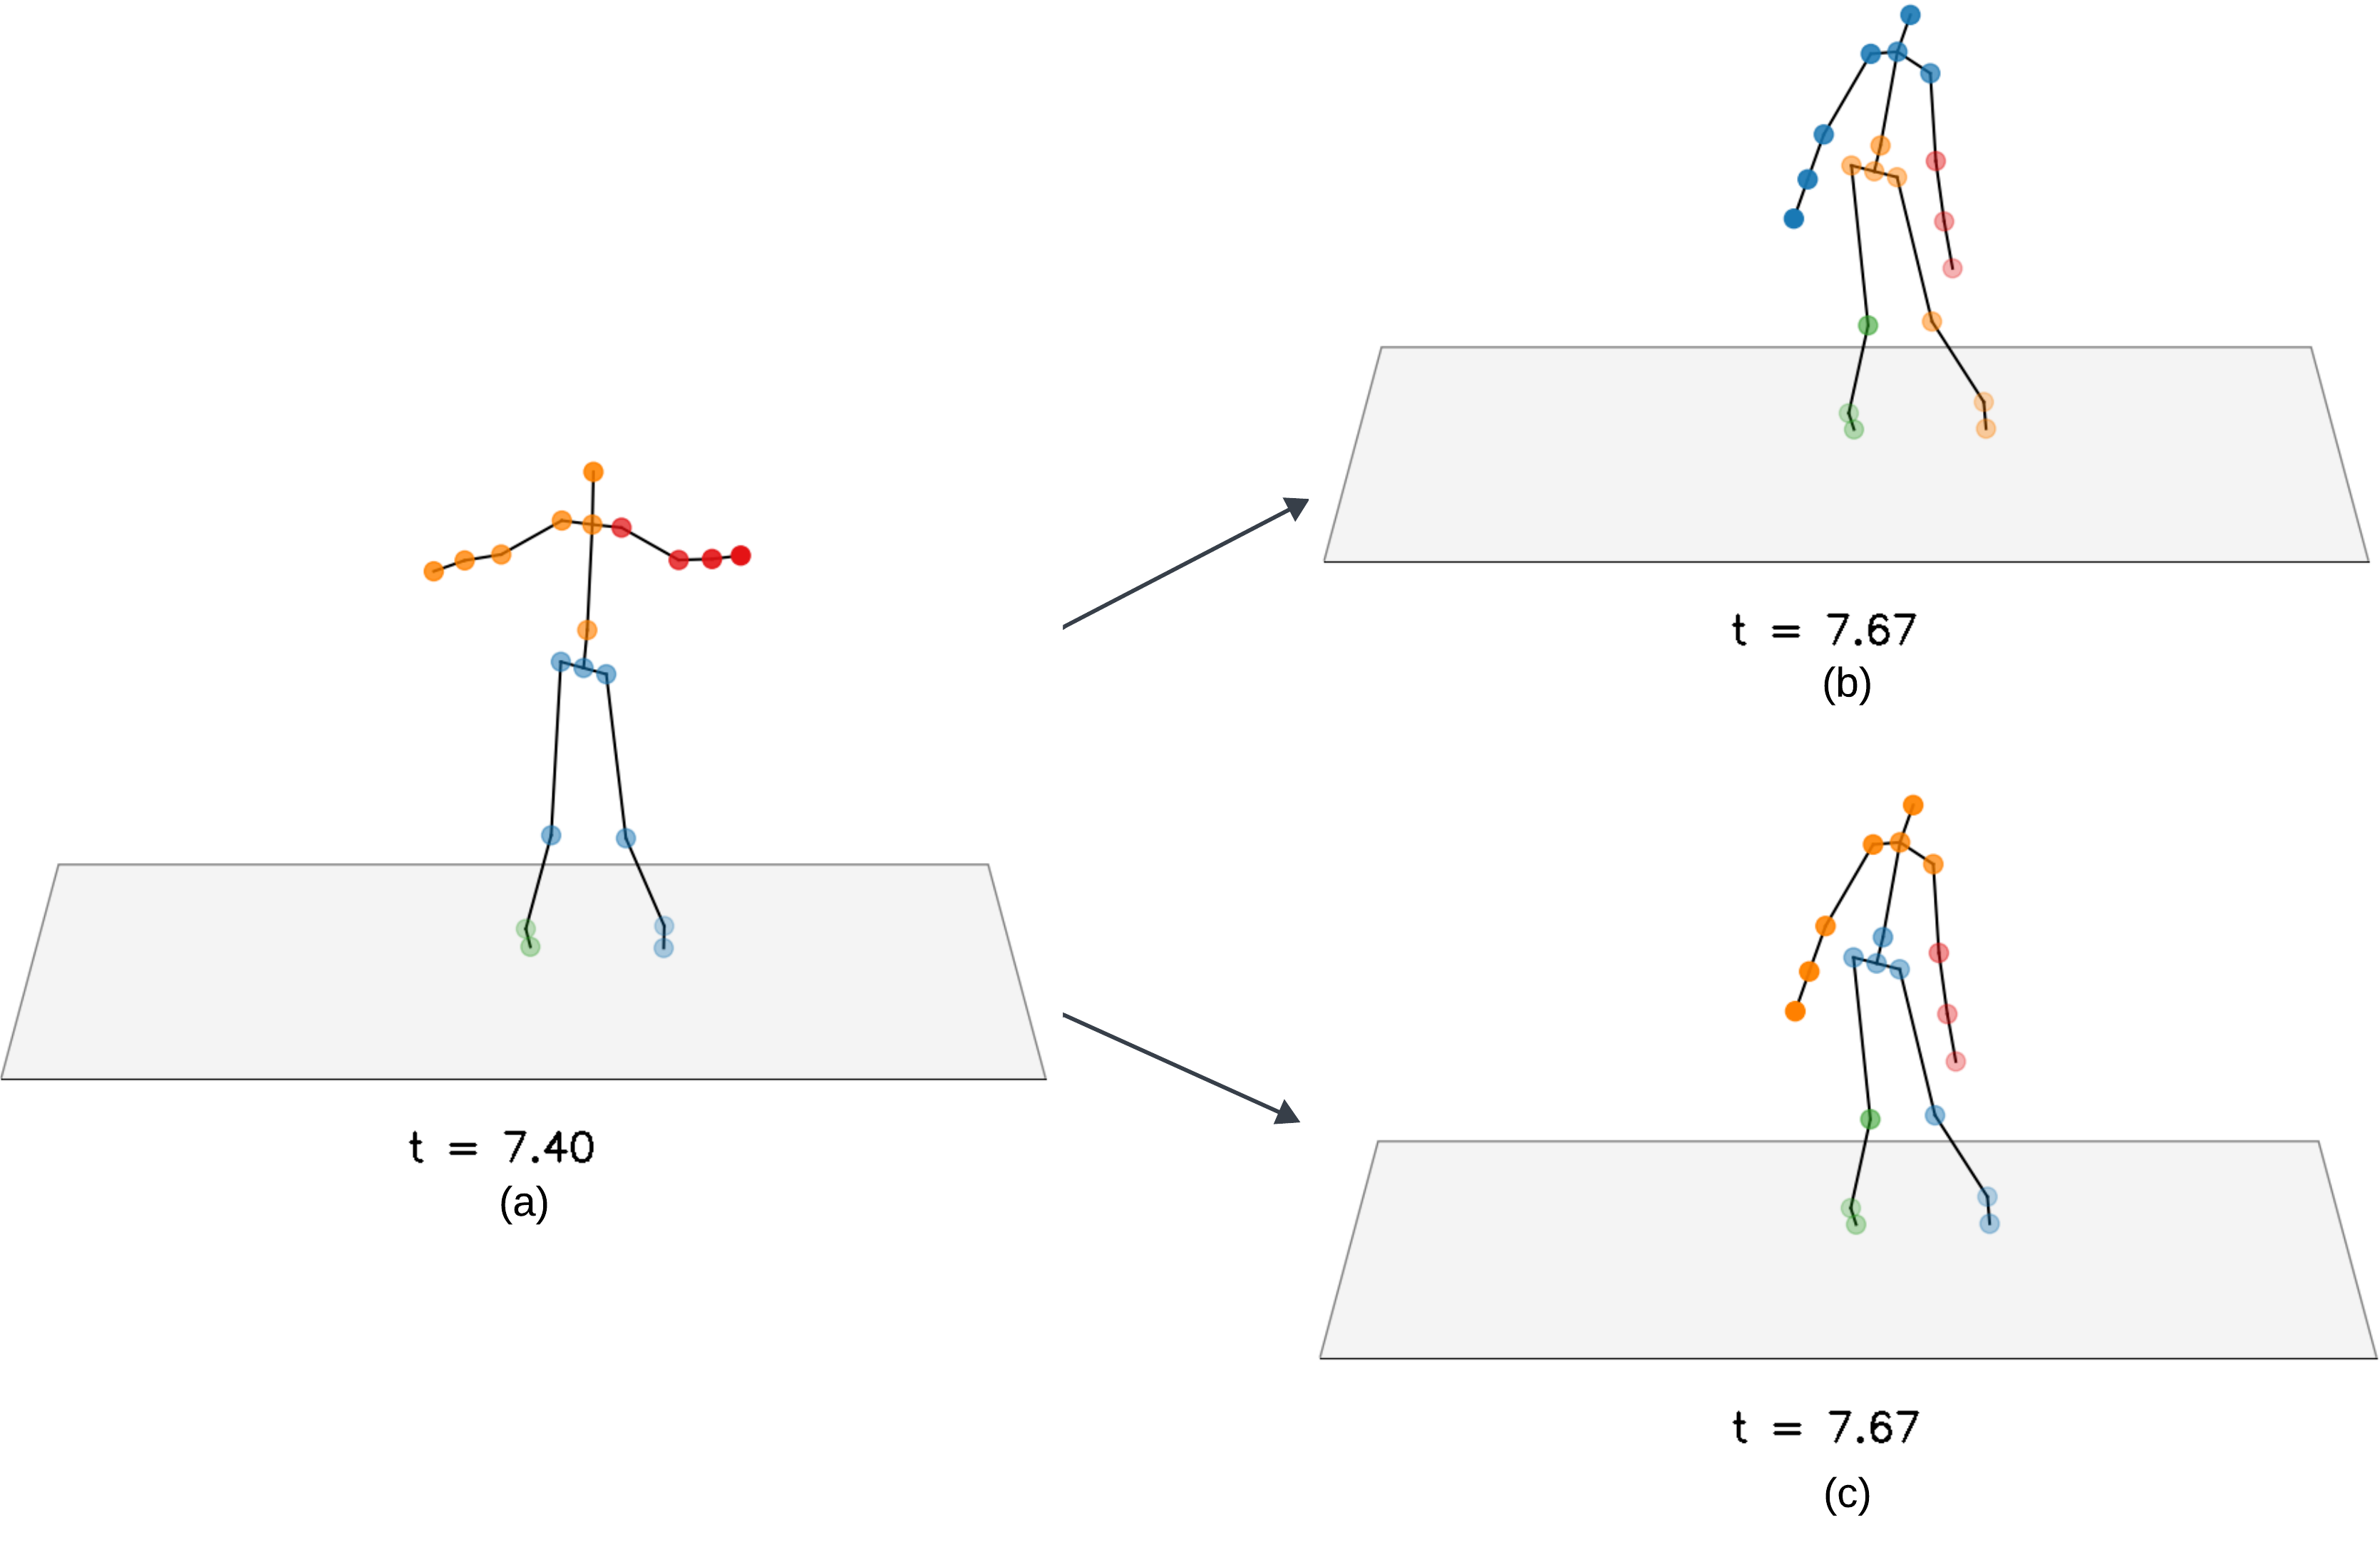
\includegraphics[width=0.99\textwidth]{graphics/ClustersStabilization.png}
  \caption{Clustering at $t=7.40$ (a), $t=7.67$ unstabilized (b), and $t=7.67$ stabilized (c).}
  \label{fig:stabilization_results}
\end{figure}

To better visualize the results achieved through stabilization, you can refer to a QR code \ref{fig:QRcode} that leads to a GIF image where the entire motion, as previously seen in Figure \ref{fig:stabilization_results}, can be observed.

\begin{figure}[H]
  \centering
  
\includegraphics[width=0.50\textwidth]{graphics/qrcode.png}
  \caption{QRcode to the GIF}
  \label{fig:QRcode}
\end{figure}

As evident from the GIF, the dancer begins from a stance with slightly spread legs and the left arm raised upwards.
Throughout the movement, the left arm descends while moving backward, the torso leans forward, taking the right arm along with it, and the left foot lifts off the ground, taking a step backward.